% !TeX spellcheck = cs_CZ
%{\tikzset{external/prefix={tikz/FYZI/}}
% \tikzset{external/figure name/.add={ch25_}{}}
%=========================== Kapitola: Lineární systémy. Přehled ==================================
\setchaptertoc
\chapter{Lineární systémy. Přehled}\label{fyz:IchapXXV}

  \section{Lineární diferenciální rovnice}\label{fyz:IchapXXVsecI}
    V této kapitole se budeme zabývat určitými aspekty oscilačních soustav, jež platí jaksi 
    obecněji a nejen ve zvláštních systémech, o nichž jsme hovořili. Pro náš konkrétní systém jsme 
    řešili 
    diferenciální rovnici
    \begin{equation}\label{fyz:eq338}
      m\dder{x}{t} + \gamma m\der{x}{t} + m\omega^2_0x = F(t).
    \end{equation}
    
    Tato konkrétní kombinace „operací“ působících na proměnnou \(x\) má zajímavou vlastnost. Když 
    za \(x\) dosadíme \((x + y)\), dostaneme součet stejných operací působících na \(x\) a na 
    \(y\); všude vynásobíme-li \(x\) konstantou \(a\), dostaneme stejnou kombinaci operací 
    \(a\)-krát. Lze to snadno dokázat. Aby nás psaní všech těchto písmen v (\ref{fyz:eq338}) 
    neunavovalo, použijeme místo toho symbol \(\mathcal{L}(x)\). Když ho někde uvidíme, je třeba si 
    místo něho představit levou stranu (\ref{fyz:eq338}). \(\mathscr{L}(x + y)\) bude při takovém 
    způsobu psaní znamenat
    \begin{equation}\label{fyz:eq339}
      \mathscr{L}(x + y) = m\dder{(x + y)}{t} + \gamma m\der{(x + y)}{t} + m\omega^2_0(x + y).
    \end{equation}
    \(\mathscr{L}\) někdy nazýváme operátorem, ale na pojmenování nezáleží, je to prostě „zkratka“. 
    Naše první tvrzení bylo, že
    \begin{equation}\label{fyz:eq340}
      \mathscr{L}(x + y) = \mathscr{L}(x) + \mathscr{L}(y),
    \end{equation}
    což samozřejmě vyplývá z faktu, že \(a(x + y) = ax + ay\), \(\der{(x + y)}{t} = \der{x}{t} + 
    \der{y}{t}\), atd. 
    
    Naše druhé tvrzení se týkalo konstanty \(a\)
    \begin{equation}\label{fyz:eq341}
      \mathscr{L}(ax) = a\mathscr{L}(x).
    \end{equation}
    Vztahy (\ref{fyz:eq340}) a (\ref{fyz:eq341}) spolu velmi těsně souvisí, neboť kdybychom do 
    (\ref{fyz:eq339}) dosadili \(x + x\), měli bychom totéž, jako když v (\ref{fyz:eq341}) bude \(a 
    = 2\) apod.
    
    V komplikovanějších problémech se může vyskytnout více derivací a \(\mathscr{L}\) může 
    obsahovat více členů. Je zajímavé vědět, zda obě rovnice (\ref{fyz:eq340}) a (\ref{fyz:eq341}) 
    zůstanou v platnosti nebo ne. Jestliže ano, nazýváme takový problém lineárním. Abychom lépe 
    ocenili obecnost některých výsledků, jež jsme dostali při analýze naší konkrétní rovnice, 
    budeme se v této kapitole věnovat některým vlastnostem lineárních systémů.
    
    Začneme studiem některých vlastností lineárních diferenciálních rovnic, když už jsme je 
    ilustrovali na konkrétní rovnici (\ref{fyz:eq338}), jíž jsme se tak podrobně zabývali. První 
    zajímavá vlastnost je tato. Předpokládejme, že máme vyřešit diferenciální rovnici pro 
    přechodový jev - vlastní kmity bez budicí síly. Chceme tedy řešit rovnici
    \begin{equation}\label{fyz:eq342}
      \mathscr{L}(x) = 0.
    \end{equation}
    
    Předpokládejme, že nějakým způsobem jsme našli určité řešení a označme ho \(x_1\), tj. máme 
    \(x_1\), pro které \(\mathscr{L}(x_1) = 0\). Vidíme, že i \(ax_1\) je řešením této rovnice. 
    Naše částečné řešení můžeme vynásobit jakoukoli konstantou a dostaneme nové řešení. Jinými 
    slovy, máme-li pohyb určité „velikosti“, je dvojnásobně „velký“ pohyb opět řešením. Plyne to 
    okamžitě z toho, že \(\mathscr{L}(ax) = a\mathscr{L}(x) = a \cdot 0 = 0\).
    
    Dále předpokládejme, že jsme nějak našli nejen jedno řešení \(x_1\), ale i druhé řešení 
    \(x_2\). (Vzpomeňme si, že když jsme při hledání přechodových jevů dosadili \(x =e^{i\alpha 
    t}\), našli jsme dvě hodnoty pro \(\alpha\), tj. dvě řešení \(x_1\) a \(x_2\)) Nyní ukažme, že 
    i kombinace \((x_1 + x_2)\) je řešením rovnice. Jinými slovy, položíme-li \(x = x_1 + x_2\), je 
    \(x\) znovu řešením rovnice. Proč? Protože je-li \(\mathscr{L}(x_1) = 0\) a \(\mathscr{L}(x_2) 
    = 0\), pak \(\mathscr{L}(x_1 + x_2) = \mathscr{L}(x_1) + \mathscr{L}(x_2) = 0 + 0 = 0\). Takže, 
    máme-li několik řešení popisujících pohyb lineární soustavy, můžeme je sčítat. 
    
    
    Zkombinujeme-li tyto dvě vlastnosti, vidíme, že můžeme sčítat třeba šest prvních řešení a dvě 
    druhá řešení; je-li \(x_1\) řešení, pak i \(\alpha x_1\) je řešení. Proto součet takovýchto 
    dvou řešení, jako například \((\alpha x_1 + \beta x_2 )\) „je rovněž řešením. Stane-li se, že 
    najdeme tři řešení, pak jakákoli kombinace těchto tří řešení znovu řešením atd. Ukazuje se, že 
    naše úloha o oscilátoru má jen dvě tzv. nezávislá řešení\footnote{Nezávislými se nazývají ta 
    řešení, jež nelze navzájem vyjádřit jako lineární kombinace.}. Počet nezávislých řešení obecně 
    závisí na tom, čemu říkáme \emph{stupně volnosti}. Nebudeme to nyní podrobně rozebírat, ale 
    máme-li diferenciální rovnici druhého řádu, existují jen dvě nezávislá řešení. My jsme našli 
    obě dvě, takže máme to nejobecnější řešení. Věnujme se dalšímu tvrzení, jež se vztahuje na 
    situaci, kdy na soustavu působí vnější síla. Předpokládejme, že příslušná nehomogenní rovnice 
    má tvar
    \begin{equation}\label{fyz:eq343}
      \mathscr{L}(x) = F(t),
    \end{equation}
    a předpokládejme, že jsme našli její partikulární řešení. Petrovo řešení nechť je \(x_P\) a 
    platí \(\mathscr{L}(x_P) = F(t)\). Předpokládejme, že chceme najít ještě jiné řešení, a že k 
    Petrovu řešení přidáme jedno z řešení homogenní rovnice pro vlastní kmity (\ref{fyz:eq342}) 
    (tj. s nulou na pravé straně), řekněme \(x_1\). Pak podle (\ref{fyz:eq340}) vidíme, že
    \begin{equation}\label{fyz:eq344}
      \mathscr{L}(x_P + x_1) = \mathscr{L}(x_P) + \mathscr{L}(x_1) = F(t) + 0 = F(t),
    \end{equation}
    
    Proto když „vynucenému“ řešení nehomogenní rovnice přidáme jakékoli „volné“ řešení homogenní 
    rovnice, opět dostaneme řešení, jež vyhovuje nehomogenní rovnici. Volné řešení pro vlastní 
    kmity se nazývá i přechodovým řešením. 
    
    Nepůsobí-li na soustavu síla, a najednou začne působit, nedostaneme ihned ustálené řešení ve 
    tvaru sinusové vlny, ale na nějaký čas se projeví přechodový jev, jenž se dříve nebo později 
    utlumí. Vynucené řešení se neutlumí, neboť je udržováno v chodu vnější silou. Nakonec za 
    dlouhou dobu zůstane jen jedno řešení, ale zpočátku se za různých okolností projeví různé 
    pohyby v závislosti na počátečních podmínkách.
    
  \section{Superpozice řešení}\label{fyz:IchapXXVsecII}
    Dostáváme se k dalšímu zajímavému tvrzení. Předpokládejme, že máme nějakou budicí sílu \(F_a\) 
    (řekněme, že osciluje s \(\omega = \omega_a\), ale naše závěry budou platit pro jakoukoli 
    funkci \(F_a\)), a že jsme našli její odpovídající vynucené řešení (nezáleží na tom, zda s 
    přechodovými řešeními nebo bez nich). Předpokládejme dále, že máme nějakou sílu \(F_b\) a znovu 
    vyřešíme celou úlohu pro tuto novou sílu. Někdo pak může přijít a říci: „Mám pro vás novou 
    úlohu k řešení. Já mám sílu \(F_a + F_b\)“ Známe řešení? Samozřejmě, že známe, neboť řešení je 
    dáno součtem dvou řešení \(x_a\), a \(x_b\), když síly působily každá zvlášť. To je skutečně 
    pozoruhodná věc. Na základě (\ref{fyz:eq340}) máme
    \begin{equation}\label{fyz:eq345}
      \mathscr{L}(x_a + x_b) = \mathscr{L}(x_a) + \mathscr{L}(x_b) = F_a(t) + F_b(t).
    \end{equation}
    
    To je příklad tzv.\textbf{ principu superpozice} pro lineární soustavy a je velmi důležitý. 
    Znamená, že máme-li složitou sílu, kterou lze vhodně rozložit na součet jednotlivých částí, z 
    nichž každá je jednoduchá v tom smyslu, že pro každou z nich, umíme vyřešit pohybovou rovnici, 
    známe řešení pro celou sílu, neboť můžeme prostě složit jednotlivá řešení stejným způsobem, 
    jakým se celková síla skládá z jednotlivých složek (obr. \ref{fyz:fig0293}).

    \begin{figure}[ht!] %\ref{fyz:fig0293}
      \centering
      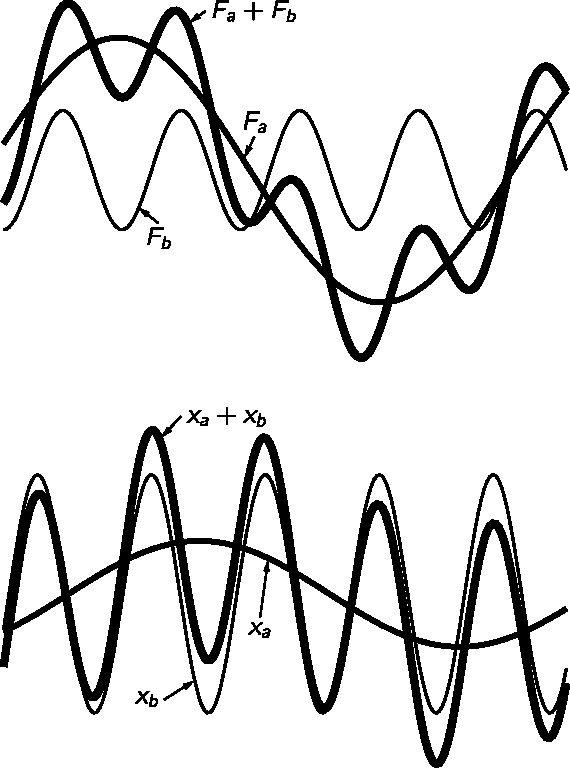
\includegraphics[width=0.7\linewidth]{fyz_fig0293.pdf}
      \caption{Příklad principu superpozice pro lineární soustavy
               (\cite[s.~334]{Feynman01})}
      \label{fyz:fig0293}
    \end{figure}
    
    Uveďme další příklad na princip superpozice. V kap. \ref{fyz:IchapXII} jsme uvedli, že jedním 
    významným faktem zákonů elektřiny je, že máme-li nějaké rozdělení nábojů \(q_a\), a vypočítáme 
    intenzitu elektrického pole \(\vec{E}_a\), v bodě \(P\) a na druhé straně máme jinou soustavu 
    nábojů \(q_b\) a vypočítáme pole \(\vec{E}_b\), v témž bodě, pak jsou-li obě soustavy nábojů 
    přítomny současně, intenzita pole \(\vec{E}\) v bodě \(P\) je rovna součtu \(\vec{E}_a\) od 
    jedné soustavy nábojů plus \(\vec{E}_b\), od druhé soustavy nábojů. Jinak řečeno, známe-li pole 
    vyvolané jedním nábojem, je pole vyvolané mnoha náboji rovno vektorovému součtu polí od 
    jednotlivých nábojů. To je přesná analogie tvrzení, že známe-li výsledek pro dvě dané síly 
    samostatně, je řešení pro sílu rovnou součtu těchto dvou sil rovno součtu jednotlivých řešení.
    
    Důvod, proč to platí v elektřině, je ten, že základní zákony elektřiny - \emph{Maxwellovy 
    rovnice} určující elektrické pole, jsou diferenciálními rovnicemi, jež jsou lineární, tj. mají 
    vlastnost (\ref{fyz:eq340}). Síle odpovídají náboje vytvářející elektrické pole a rovnice pro 
    výpočet pole z náboje je lineární. 

    \begin{figure}[ht!] %\ref{fyz:fig0294}
      \centering
      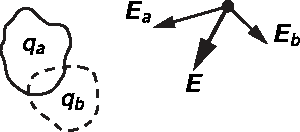
\includegraphics[width=0.6\linewidth]{fyz_fig0294.pdf}
      \caption{Princip superpozice v elektrostatice
               (\cite[s.~335]{Feynman01})}
      \label{fyz:fig0294}
    \end{figure}
    
    Jako další příklad si položme otázku, jak je možné v rádiu naladit stanici, když současně 
    vysílá mnoho jiných stanic. Radiovysílač v podstatě vysílá oscilující elektrické pole velmi 
    vysoké frekvence, které působí na anténu našeho rádia. Je pravda, že amplituda oscilace pole se 
    mění, je modulována hlasovým signálem, ale tyto změny jsou velmi pomalé a nebudeme se jimi 
    znepokojovat Když slyšíme: „Tato stanice vysílá na frekvenci 780 kilocyklů“, znamená to, že 
    frekvence oscilací elektrického pole vysílací antény je 780 000 oscilací za sekundu a toto pole 
    vyvolává kmity elektronů v naší anténě s touto frekvencí. Ve stejném okamžiku může ve stejném 
    městě vysílat jiná radiostanice frekvencí, řekněme, 550 kilocyklů za sekundu a elektrony v naší 
    anténě budou kmitat i touto frekvencí. Je otázka, jak lze oddělit signály dopadající na jedno 
    rádio s frekvencí 780 kilocyklů od signálů s frekvencí 550 kilocyklů? Určitě neslyšíme obě 
    stanice současně. 
    
    \begin{figure}[ht!] %\ref{fyz:fig0295}
      \centering
      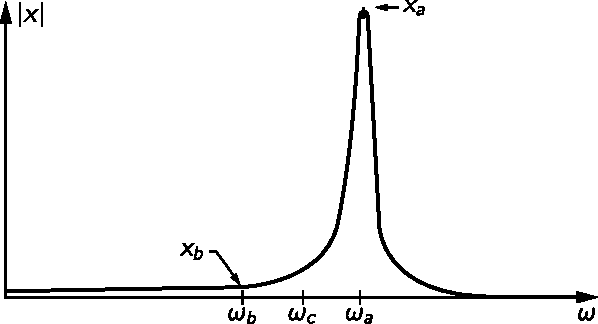
\includegraphics[width=0.7\linewidth]{fyz_fig0295.pdf}
      \caption{Ostře vyladěná rezonanční křivka
               (\cite[s.~335]{Feynman01})}
      \label{fyz:fig0295}
    \end{figure}
    
    Podle principu superpozice vznikne v rádiu, jehož první část tvoří lineární obvod, pod vlivem 
    elektrického pole \(F_a + F_b\) proud \(x_a + x_b\). Zdálo by se, že jednotlivá řešení nikdy 
    nerozlišíme. Právě podle principu superpozice se zdá, že se nikdy nevyhneme tomu, aby byla 
    přítomna obě současně. Ale vzpomeňme si, že pro rezonanční obvod má křivka závislosti \(x\) 
    (připadajícího na jednotku \(F\)) na frekvenci tvar jako na obr. \ref{fyz:fig0295}. Má-li 
    vstupní obvod velmi vysoké \(Q\), bude mít křivka ostré maximum. Předpokládejme, že obě stanice 
    jsou srovnatelně silné; obě síly mají stejnou amplitudu. Výsledný signál je roven součtu 
    \(x_a\) a \(x_b\), Ale \(x_a\), na obr. \ref{fyz:fig0295} je obrovské, zatímco \(x_b\) je malé. 
    Takže navzdory tomu, že oba signály mají zpočátku stejnou intenzitu, po průchodu kvalitním 
    rezonačním obvodem v rádiu naladěném na \(\omega_a\), (tj. frekvenci jedné ze stanic) je signál 
    této stanice mnohem silnější než druhý signál. Při působení obou vysílačů se proto výsledný 
    signál skládá téměř výlučně z \(\omega_a\) - vyladili jsme požadovanou stanici.
    
    Jak se vlastně stanice naladí? Ladí se tak, že změnou \(L\) nebo \(C\) v obvodu měníme 
    \(\omega_0\) jež závisí na \(L\) a \(C\). Většina rádií je zkonstruována tak, že se mění 
    kapacita. Když přeladíme rádio, bude ukazatel stanic v nové poloze. Tím dosáhneme toho, že 
    rezonanční frekvence obvodu se posune například do \(\omega_c\). V tom případě neslyšíme ani 
    jednu stanici: je ticho, samozřejmě za předpokladu, že žádná jiná stanice nevysílá na frekvenci 
    \(\omega_c\). Měníme-li dále kapacitu, až se rezonanční křivka dostane do \(\omega_b\) uslyšíme 
    druhou stanici. Toto je princip ladění rádia - využívá se přitom princip \emph{superpozice a 
    rezonance}\footnote{V modemích superheterodynových přijímačích je ladění složitější. Všechny 
    stupně jsou naladěny na konstantní frekvenci (tzv. mezifrekvenci MF) a vstupní signál se 
    směšuje v nelineámím obvodu s frekvencí laditelného oscilátoru, čímž vzniká nová frekvence 
    (rozdíl frekvencí vstupního signálu a laditelného oscilátoru), jež je rovna mezifrekvenci, a ta 
    se pak zesiluje. Budeme se tím zabývat v kap. \ref{fyz:IchapL}.}.
    
    Na závěr popišme kvalitativně, co se stane, je-li budicí síla velmi komplikovaná. Z množství 
    možných způsobů existují dva, zvlášť užitečné, obecné způsoby řešení takovéhoto problému. Jeden 
    je tento: Předpokládejme, že problém umíme vyřešit pro určité známé síly, jako jsou například 
    síly s funkcí sinus ideálním průběhem různých frekvencí. Víme, že najít řešení pro sinové vlny 
    je „dětská hračka“. Máme tedy tzv. „dětské“ případy. Otázkou je, zda by nebylo možné naši 
    komplikovanou sílu vyjádřit jako součet dvou nebo více takových „dětských“ sil. Na obr. 
    \ref{fyz:fig0294} jsme měli již dost komplikovanou křivku a mohli bychom ji udělat ještě 
    složitější, kdybychom přidali další sinové vlny. Takže zcela určitě lze takto získat velmi 
    komplikované křivky. Stejně platí i opačné tvrzení: Prakticky každou křivku lze získat složením 
    \emph{nekonečného počtu} sinových vln rozličných délek (nebo frekvencí), přičemž pro každou z 
    nich známe řešení. Potřebujeme vědět jen to, kolik musíme vzít z každé sinové vlny, abychom 
    dostali dané \(F\), takže pak se řešení \(x\) skládá ze součtu sinových vln, přičemž každá je 
    vynásobena příslušným efektivním poměrem \(x\)k  \(F\). Tato metoda řešení se nazývá 
    \textbf{metodou Fourierových transformací} nebo \textbf{Fourierova analýza}. Tuto analýzu teď 
    nebudeme provádět, chtěli jsme jen naznačit její princip.
    
    Druhý, velmi zajímavý způsob, jak lze řešit náš problém, je následující. Předpokládejme, že po 
    těžké duševní námaze by se nám podařilo vyřešit náš případ pro speciální sílu ve tvaru krátkého 
    impulzu - síla se rychle zapne a zase vypne, a to je všechno. Stačí najít řešení jen pro impulz 
    nějaké jednotkové velikosti a pro všechny jiné impulzy ho dostaneme, když ho vynásobíme 
    příslušným faktorem. Víme, že řešením \(x\) pro nějaký impulz jsou tlumené kmity. Co umíme říci 
    o řešení pro nějakou sílu, jaká je například na obr. \ref{fyz:fig0296}?

    \begin{figure}[ht!] %\ref{fyz:fig0296}
      \centering
      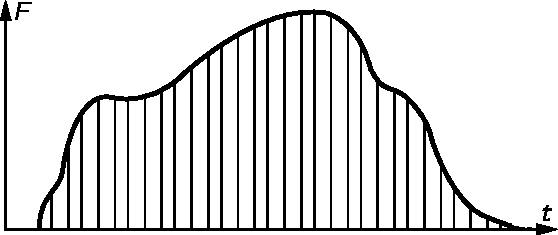
\includegraphics[width=0.7\linewidth]{fyz_fig0296.pdf}
      \caption{Na složitou sílu se lze dívat jako na sled ostrých pulzů
               (\cite[s.~337]{Feynman01})}
      \label{fyz:fig0296}
    \end{figure}
    
    Takovou sílu lze přirovnat k celé řadě úderů kladivem. Nejdříve síla není, pak najednou působí 
    stálá síla - impulz, impulz, impulz, impulz, ... a pak přestane. Spojitou sílu si tedy 
    představíme jako sérii impulzů následujících těsně za sebou. Výsledek pro jeden impulz známe, 
    takže pro celou sérii impulzů dostaneme výsledek jako celou sérii tlumených oscilací. Bude to 
    křivka odpovídající prvnímu impulzu, pak (o něco později) k ní přičteme křivku druhého impulzu, 
    pak třetího atd. Tak umíme matematicky vyjádřit úplné řešení pro libovolné funkce, známe-li 
    řešení pro nějaký impulz. Řešení pro libovolnou sílu dostaneme prostě integrací. Je to tzv. 
    \textbf{metoda Greenových funkcí}. Greenova funkce je řešením pro impulz a metoda analýzy 
    pomocí skládání řešení pro impulzy se nazývá metodou Greenových funkcí.
    
    Fyzikální principy obsažené v obou těchto schématech jsou jednoduché - jde jen o lineární 
    rovnice - lze je snadno pochopit. Ale matematické problémy s tím spojené (komplikované 
    integrace apod.) jsou pro nás zatím dost obtížné, abychom se jim nyní věnovali. Vrátíte se k 
    nim nejpravděpodobněji poté, co budete lépe ovládat matematiku. Ale podstata je tu skutečně 
    velmi jednoduchá.
    
    Nakonec ještě několik poznámek o tom, proč jsou lineární systémy tak důležité. Odpověď 
    jejednoduchá: Protože je umíme řešit! Proto většinou řešíme lineární problémy. Jak se ukazuje, 
    je druhý a nejdůležitější důvod ten, že základní fyzikální zákony jsou často lineární. 
    Například Maxwellovy rovnice zákonů elektřiny jsou lineární. Velké zákony kvantové mechaniky, 
    jak se zatím ukazuje, jsou vyjádřeny rovněž lineárními rovnicemi. Proto jsme věnovali tolik 
    času lineárním rovnicím. Rozumíme-li lineárním rovnicím, můžeme v zásadě pochopit mnoho věcí.
    
    Zmíníme se ještě o jedné situaci, kdy se rovněž setkáváme s lineárními rovnicemi. Při malých 
    výchylkách lze mnohé funkce lineárně aproximovat. Například, přesná pohybová rovnice obyčejného 
    kyvadla je
    
    \begin{equation}\label{fyz:eq346}
      \dder{\vartheta}{t} = - \left(\dfrac{g}{L}\right)\sin\vartheta
    \end{equation}
    
    Tuto rovnici lze řešit pomocí \emph{eliptických funkcí}, ale nejsnadněji ji vyřešíme numericky, 
    jak jsme to uvedli v kap. \ref{fyz:IchapIX} u \emph{Newtonových zákonů pohybu}. Nelineární 
    rovnici nelze obvykle řešit jinak, než numericky. Pro malé \(\vartheta\) je \(sin\vartheta\) 
    prakticky rovno \(\vartheta\), takže pak máme lineární rovnici. Ukazuje se, že malé efekty jsou 
    často lineární - například pohyb kyvadla při malých úhlech. Jako další příklad vzpomeňme 
    pružinu. Jestliže ji mírně natahujeme, je síla úměrná jejímu prodloužení. Zatáhneme-li za ni 
    silně, přetrhne se a síla je zcela jinou funkcí vzdálenosti! Lineární rovnice jsou důležité. Ve 
    skutečnosti jsou tak důležité, že snad padesát procent času ve fyzice a v technice věnujeme 
    řešení lineárních rovnic.
    
  \section{Oscilace v lineárních systémech}\label{fyz:IchapXXVsecIII}
    Nyní shrňme to, o čem jsme hovořili v několika posledních kapitolách. Fyziku kmitavých pohybů 
    lze velmi snadno zastínit matematikou. Je to velmi jednoduchá fyzika, a zapomeneme-li na chvíli 
    na matematiku, uvidíme, že dokážeme pochopit téměř všechno, co se děje v kmitavých soustavách. 
    Zaprvé, máme-li pružinu se závažím, velmi snadno lze pochopit, proč systém kmitá - je to 
    následek setrvačnosti. My stáhneme závaží dolů a pružina ho vytáhne zpět nahoru; když prochází 
    nulou, svou rovnovážnou polohou, nemůže se najednou zastavit; protože má určitou hybnost, 
    pokračuje v pohybu až se vychýlí na druhou stranu, a tak se pohybuje sem a tam, takže kdyby 
    neexistovalo tření, mohli bychom očekávat kmitavý pohyb, jenž skutečně také nastává. 
    Existuje-li však sebemenší tření, nebude výchylka na zpáteční dráze tak velká, jako na začátku.
    
    Co se děje v cyklech následujících za sebou? Závisí to na druhu tření a na velikosti tření. 
    Předpokládejme, že vymyslíme takové tření, jež se při změně amplitudy mění ve stejném poměru k 
    ostatním silám, setrvačné síle a síle pružiny. Jinak řečeno, pro malé kmity by mělo být tření 
    slabší než pro velké kmity. Obyčejné tření nemá tuto vlastnost, takže by muselo jít o nějaký 
    nový druh tření, které by bylo úměrné výchylce, proto pro velké kmity by bylo silnější a pro 
    malé kmity slabší. Kdybychom měli tření takového druhu, nacházel by se systém po každém 
    následujícím cyklu ve stejném stavu, jako byl na začátku, jenže o něco menším. Všechny síly se 
    zmenšily ve stejném poměru: síla pružiny je slabší, vliv setrvačnosti je menší, neboť zrychlení 
    jsou menší a tření je samozřejmě rovněž menší. Zjistíme, že při takovém druhu tření je každý 
    kmit přesně stejný jako byl první kmit, jenomže má menší amplitudu. Jestliže za dobu prvního 
    cyklu klesla amplituda, řekněme, na 90\% toho, jaká byla na začátku, pak za dobu dalšího cyklu 
    klesne na 90\% z 90\% atd. \emph{- velikosti kmitů se po každém cyklu zmenší ve stejném 
    poměru}. Tomuto průběhu vyhovuje exponenciála. Za stejný časový interval se změní ve stejném 
    poměru. Znamená to, že je-li poměr amplitudy k amplitudě v předcházejícím cyklu \(a\), bude 
    následující amplituda dána poměrem \(a^2\), ještě delší \(a^3\). Takže amplituda je rovna 
    nějaké konstantě umocněné na počet prošlých cyklů:
    \begin{equation}\label{fyz:eq347}
      A = A_0a^n.
    \end{equation}

    \begin{figure}[ht!] %\ref{fyz:fig0297}
      \centering
      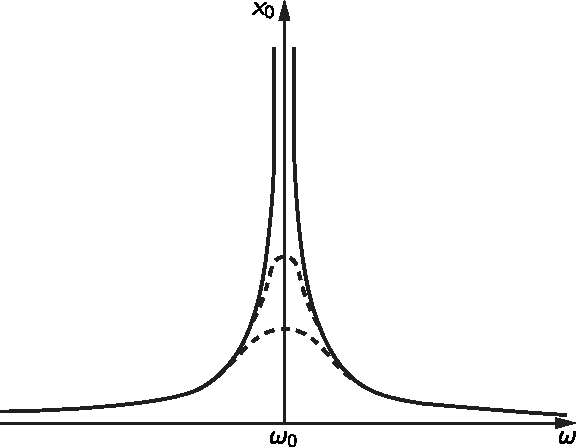
\includegraphics[width=0.7\linewidth]{fyz_fig0297.pdf}
      \caption{Rezonančí křivky za přítomnosti různých velikostí tření 
               (\cite[s.~427]{Feynman01})}
      \label{fyz:fig0297}
    \end{figure}
    
    Ale samozřejmě, že \(n\) je úměrné \(t\), takže je zcela jasné, že obecným řešením budou nějaké 
    oscilace (sinus nebo kosinus \(\omega t\)) krát amplituda, která se mění víceméně jako \(b^t\), 
    ale \(b\) lze napsat jako \(e^{-c}\) pro \(b\) kladné a menší než \(1\). Takže to je důvod, 
    proč má řešení tvar \(e^{-ct}\cos\omega t\). Je to velmi prosté.
    
    Co se stane, když tření nebude tak umělé; například obyčejné tření o stůl, takže tření je 
    konstantní a nezávislé na velikosti oscilací, jež mění svůj směr po každém polocyklu? V tom 
    případě už rovnice není lineární, těžko ji lze řešit, a proto je třeba ji řešit numerickou 
    metodou uvedenou v kap. \ref{fyz:IchapIX} nebo zvlášť pro každý polocyklus. Numerická metoda je 
    nejúčinnější ze všech. Umožňuje vyřešit jakoukoli rovnici. Matematickou analýzu můžeme použít 
    jen u jednoduchých problémů.
    
    Matematická analýza není tak ohromný nástroj, jak se často říká; řeší jen nejednodušší možné 
    rovnice. Jakmile se rovnice stávají jen o trochu komplikovanějšími, nelze je řešit analyticky. 
    Numerická metoda, s níž jsme se seznámili na začátku přednášek, dokáže vyřešit jakoukoli 
    fyzikálně zajímavou rovnici.
    
    Co lze říci o rezonanční křivce? Proč existuje rezonance? Představme si na okamžik, že není 
    tření, a že máme nějaké kyvadlo, jež může kývat samo od sebe. Ťukneme-li do kyvadla vždy v 
    pravou chvíli, můžeme ho dostat do prudkých oscilací. Co se však stane, zavřeme-li oči a budeme 
    do něho ťukat v libovolných pravidelných intervalech? Stane se, že někdy do něho ťukneme právě 
    tehdy, kdy jde špatným směrem. Když se nám podaří najít správný rytmus, každé ťuknutí se 
    uskuteční v pravý okamžik a kmity budou větší a větší. Takže za nepřítomnosti tření dostaneme 
    závislost na frekvenci, která je podobná plné čáře na obr. \ref{fyz:fig0297}. Kvalitativně jsme 
    pochopili rezonanční křivku; abychom dostali její přesný tvar, je třeba si pomoci matematikou. 
    Křivka stoupá do nekonečna pro \(\omega\rightarrow\omega_0\). kde \(\omega_0\) je \emph{vlastní 
    frekvence oscilátoru}.
    
    Nyní předpokládejme, že na oscilátor působí slabé tření. Při malých výchylkách se jeho vliv 
    příliš neprojeví. Rezonanční křivka je stejná, vyjma oblasti blízko rezonance. Místo toho, aby 
    v blízkosti rezonance stoupala do nekonečna, stoupne tak, že práce, kterou vykonáme při každém 
    ťuknutí, kompenzuje ztráty v důsledku tření při každém cyklu. Vrchol křivky je proto zaoblený - 
    nejde do nekonečna. Při větším tření se vrchol křivky zaoblí ještě více. Někdo může říci: 
    „Myslel jsem si, že šířky křivek závisí na velikosti tření.“ Je to proto, že obvykle se tyto 
    křivky kreslí tak, že se bere jako jednotková jejich výška. Jejich matematické vyjádření lze 
    snadněji pochopit, jestliže se všechny nakreslí ve stejném měřítku - jediné, co tření způsobí 
    je, že se sníží jejich maxima! Je-li tření menší, vrcholek se poněkud zvedne a křivka se stane 
    užší.
    
    Nakonec si vezmeme případ, kdy je tření velmi velké. Je-li tření příliš velké, systém vůbec 
    neosciluje. Energie pružiny sotva stačí k překonání tření, takže systém se pomalu vrátí do 
    rovnovážné polohy.
    
  \section{Analogie ve fyzice}\label{fyz:IchapXXVsecIV}
    V tomto přehledu chceme ještě poukázat na to, že závaží a pružiny nejsou jedinými lineárními 
    systémy, ale že existují i jiné lineární systémy. Tak například existují určité elektrické 
    systémy, tzv. \emph{lineární obvody}, které tvoří úplnou analogii mechanických systémů. Zatím 
    jsme přesně nevysvětlili, proč se jednotlivé prvky v elektrickém obvodu chovají tak, jak se 
    chovají - v tuto chvíli nás to nezajímá. Že se chovají tak, jak jsme uvedli, je experimentálně 
    ověřitelný fakt.
    
    Vezměme nejjednodušší možný příklad. Mějme kousek drátu, což je vlastně nějaký odpor, a 
    připojme ho na nějaký rozdíl potenciálů \(U\). Smysl \(U\) je tento: přeneseme-li náboj \(q\) z 
    jednoho konce drátu na druhý konec, je vykonaná práce rovna \(qU\). Čím je vyšší napětí, tím 
    větší práce se vykonala při přechodu nábojů z konce drátu s vysokým potenciálem na konec s 
    nízkým potenciálem. Takže náboje při přechodu z jednoho konce na druhý uvolňují energii. Náboje 
    však prostě neproběhnou z jednoho konce drátu na druhý; atomy v drátu představují pro proud 
    určitý odpor, přičemž téměř pro všechny běžné látky platí zákon: proud \(I\), tj. určité 
    množství nábojů, jež projde vodičem za jednotku času, je úměrné tomu, jaká síla na ně 
    působí - jinými slovy, je úměrné velikosti přiloženého napětí
    \begin{equation}\label{fyz:eq348}
      U = IR = R\der{q}{t}.
    \end{equation}
    
    Koeficient \(R\) se nazývá \emph{odpor} a uvedená rovnice \emph{Ohmův zákon}. Jednotkou 
    odporuje jeden \emph{ohm}; je roven jednomu \emph{voltu na ampér}. V mechanice lze takovou sílu 
    tření úměrnou rychlosti těžko realizovat; ale v elektrických obvodech je to velmi snadné a pro 
    většinu kovů platí Ohmův zákon mimořádně přesně. 
    
    Často potřebujeme znát práci vykonanou za sekundu, neboli výkon, nebo energii uvolněnou náboji 
    postupujícím podél drátu. Přenesením náboje \(q\) napětím \(U\) se vykoná práce \(qU\), takže 
    práce vykonaná za sekundu pak bude \(Udq/dt\), což je totéž jako \(U\cdot I\) neboli \(IR\cdot 
    I=I^2R\). To je tzv. \emph{tepelný výkon} - množství tepla, jež se podle zákona zachování 
    energie uvolnilo v odporu za sekundu. Je to například teplo, které způsobuje žhavení vlákna v 
    obyčejné žárovce.
    
    Mechanické systémy mají i jiné zajímavé vlastnosti, například setrvačnou hmotnost, a ukazuje 
    se, že existuje i její elektrická analogie. Lze vyrobit takovou elektrickou součástku, tzv. 
    indukční cívku, jejíž významná vlastnost se nazývá indukčnost. Když v ní vznikne proud, nechce 
    se zastavit. K jeho změně je třeba napětí! Je-li proud stálý, na cívce napětí nevzniká, a proto 
    pro stejnosměrný proud indukčnost jakoby neexistuje. Začíná se projevovat jen při změnách 
    proudu. Platí pro ni rovnice
    \begin{equation}\label{fyz:eq349}
      U = L\der{I}{t} = L\dder{q}{t}.
    \end{equation}
    a jednotka indukčnosti je \emph{jeden henry}. Tato jednotka je definována tak, že napětí 
    jednoho voltu způsobí v cívce s indukčností jednoho henry změnu proudu jednoho ampéru za 
    sekundu. Rovnici (\ref{fyz:eq349}) můžeme považovat za analogii Newtonova zákona pro elektřinu; 
    \(U\) odpovídá \(F\). \(L\) odpovídá \(m\) a \(I\) odpovídá rychlosti! V obou systémech, v 
    mechanickém i v elektrickém, se stejně odvodí všechny další rovnice, neboť jedny z druhých 
    můžeme dostat jednoduchou záměnou odpovídajících symbolů. Vše, co odvodíme v jednom systému, 
    bude platit pro oba systémy.
    
    Co z elektřiny odpovídá mechanické pružině, pro niž se síla zvětšovala úměrně prodloužení? 
    Vyjdeme-li z rovnice \(F=kx\) a zaměníme \(F \rightarrow U\) a \(x \rightarrow q\), dostaneme 
    \(U = \alpha q\). Taková součástka existuje a je jediná ze tří prvků elektrického obvodu, 
    kterou umíme skutečně pochopit, neboť soustavu dvou paralelních desek jsme již studovali. 
    Zjistili jsme, že jestliže na deskách byly stejné náboje opačných znamének, byla intenzita 
    elektrického pole mezi nimi úměrná velikosti nábojů. Práce vykonaná přenesením jednotkového 
    náboje z jedné desky na druhou je přesně úměrná náboji na deskách. Tato práce je definicí 
    rozdílů potenciálů a je rovna dráhovému integrálu intenzity elektrického pole z jedné desky na 
    druhou. Konstanta úměrnosti se z historických důvodů neoznačuje \(C\), ale \(1/C\). Bylo by 
    dobré ji označit \(C\), ale nestalo se tak. Takže máme
    \begin{equation}\label{fyz:eq350}
      U = \frac{q}{C}.
    \end{equation}
    Jednotkou kapacity \(C\) je \emph{farad}. Náboj velikosti jednoho coulombu na každé z desek 
    jednofaradového kondenzátoru vyvolá napětí jednoho voltu.
    
    To jsou naše analogie a rovnici odpovídající rezonančnímu obvodu dostaneme přímo dosazením 
    \(L\) za \(m\), \(q\) za \(x\) atd.
    \begin{subequations}\label{fyz:eq351}
      \begin{align}
        m\dder{x}{t} + \gamma m\der{x}{t} + kx   &= F,   \label{fyz:eq351a}   \\
        L\dder{q}{t} + R\der{q}{t} + \frac{q}{C} &= U.   \label{fyz:eq351b}
      \end{align}
    \end{subequations}
    
    Vše, co jsme zjistili o (\ref{fyz:eq351a}), lze přetransformovat a aplikovat na 
    (\ref{fyz:eq351b}). Každý následek je stejný do té míry, že můžeme provést jednu skvělou věc. 
    Předpokládejme, že máme dost komplikovaný mechanický systém, nejen závaží na pružině, ale 
    několik závaží na několika pružinách, vše vzájemně propojeno. Co uděláme? Budeme řešit rovnice? 
    Lze postupovat i tak, ale můžeme sestrojit elektrický obvod, pro který budou platit stejné 
    rovnice jako pro mechanický systém! Chceme-li například analyzovat pohyb závaží na pružině, 
    proč bychom nesestrojili takový elektrický obvod, v němž použijeme indukčnost úměrnou hmotnosti 
    závaží, odpor úměrný \(m\gamma\) a \(1/C\) úměrné \(k\), vše ve stejném poměru? Takový 
    elektrický obvod bude přesnou analogií mechanického kmitavého systému v tom smyslu, že přesně 
    tak, jak se mění \(q\) v závislosti na \(U\) (přičemž \(U\) je zvoleno tak, aby mělo stejný 
    průběh jako má mechanická síla), bude se měnit \(x\) v závislosti na síle! Proto máme-li 
    komplikovaný systém s množstvím vzájemně spojených součástek, můžeme ho imitovat použitím 
    množství vzájemně spojených odporů, indukčních cívek a kondenzátorů. Jakou to má výhodu? Jeden 
    problém je přesně tak obtížný (nebo snadný) jako druhý, neboť jsou zcela ekvivalentní. Výhodou 
    není to, že by \emph{matematické rovnice} pro elektrický obvod bylo možné řešit snadněji, ale 
    to, že elektrický obvod lze snadněji \emph{sestrojit} a snadněji v něm lze něco \emph{změnit}.
    
    Předpokládejme, že jsme zkonstruovali automobil a chceme zjistit, jak se bude chvět při jízdě 
    po nějaké hrbolaté cestě. Sestavíme elektrický obvod s indukčnostmi představujícími setrvačnost 
    kol, tuhost pružin nahradíme kapacitami představujícími odpružení kol, odpory budou 
    představovat tlumiče. Ještě potřebujeme hrbolatou cestu. Tu nahradí generátor, jehož napětí 
    bude tvarováno tak, aby odpovídalo některým hrbolům na cestě, a pak můžeme sledovat, jak 
    nadskakuje levé kolo, tím, že měříme náboj na příslušném kondenzátoru. Dejme tomu, že měřením 
    (jež je velmi jednoduché) zjistíme, že kolo příliš kmitá. Potřebujeme silnější nebo slabší 
    tlumiče? Rozmontujeme takovou komplikovanou věc jako je auto, vyměníme v něm tlumiče a zkusíme 
    to znovu? Ne! Prostě otočíme knoflíkem a nastavíme na stupnici jinou hodnotu odporu; číslo 10 
    na stupnici odpovídá tlumiči č. 3, a tak zvětšíme tlumení. Kmitání se zhoršilo - v pořádku, 
    zkusíme tlumení zmenšovat. Kmitání je ještě horší; změníme tuhost pružiny (nastavením čísla 17) 
    a takto elektricky nastavíme všechny parametry obyčejným otáčením knoflíků. 
    
    Tomu se říká \emph{analogový počítač}. Je to zařízení, s jehož pomocí se systém, který chceme 
    zkoumat, modeluje jiným systémem popsaným stejnými rovnicemi. Takovéto zařízení lze snadněji 
    postavit, měřit, přizpůsobovat a zlikvidovat!
    
  \section{Sériové a paralelní impedance}\label{fyz:IchapXXVsecV}
    Nakonec tu máme ještě jeden důležitý bod, který tak úplně nepatří k tématu tohoto přehledu. 
    Týká se elektrických obvodů s více než jedním prvkem. Vidíme například, že v obvodu obsahujícím 
    indukční cívku, odpor a kondenzátor (např. na obr \ref{fyz:fig0301}) prochází náboj všemi třemi 
    prvky, takže proud v takto jedinečně propojené soustavě je stejný ve všech bodech obvodu. 
    Protože proud je v každém prvku stejný, napětí na \(R\) je \(IR\), napětí na \(L\) je 
    \(LdI/dt\) atd., takže celkový úbytek napětí je roven součtu jednotlivých napětí, což vede k 
    rovnici (\ref{fyz:eq351b}). Metodou komplexních čísel jsme našli ustálené řešení pro pohyb 
    vybuzený sinusoidální silou. Tak jsme zjistili, že \(\hat{U}=\hat{Z}\hat{I}\), kde \(\hat{Z}\) 
    je \textbf{impedance} tohoto obvodu. Znamená to, že při zapojení sinusoidálního napětí 
    \(\hat{U}\) dostaneme proud \(\hat{I}\).
    
    Nyní předpokládejme, že máme složitější obvod, skládající se ze dvou částí, jež samy mají 
    nějaké impedance \(\hat{Z}_1\) a \(\hat{Z}_2\). Zapojme je do \emph{série} a zapněme napětí 
    \(\hat{U}\) (obr. \ref{fyz:fig0298a}). Co se stane? Nyní je to o něco složitější, ale jestliže 
    proud procházející \(\hat{Z}_1\) je \(\hat{I}\), bude napětí na \(\hat{Z}_1\) rovno 
    \(\hat{U}_1=\hat{Z}_1\hat{I}\), a podobně, napětí na \(\hat{Z}_2\) bude 
    \(\hat{U}_2=\hat{Z}_2\hat{I}\). Oběma částmi teče stejný proud. Celkové napětí je pak rovno 
    součtu napětí na jednotlivých částech a máme \(\hat{U} = \hat{U}_1 + \hat{U}_2 = (\hat{Z}_1 + 
    \hat{Z}_2)\hat{I}\).

    \begin{figure}[ht!]      %\ref{fyz:fig0298}
      \centering
      \subcaptionbox{\label{fyz:fig0298a}}{\luafigure[0.45]{fyz_fig0298a.pdf}}
      \subcaptionbox{\label{fyz:fig0298b}}{\luafigure[0.45]{fyz_fig0298b.pdf}}
      \caption{Sériové a paralelní zapojení dvou impedancí \cite[s.~342]{Feynman01}}
      \label{fyz:fig0298}
    \end{figure}

    To znamená, že celkové napětí na obvodu lze napsat jako \(\hat{U}=\hat{Z}\hat{I}\), kde  
    \(\hat{Z}\) \emph{celková impedance sériového obvodu} a je rovna součtu impedancí jednotlivých 
    částí:
    \begin{equation}\label{fyz:eq352}
      \hat{Z} = \hat{Z}_1 + \hat{Z}_2.
    \end{equation}
    To není jediný způsob, jak lze zapojovat součástky. Můžeme je zapojit i \emph{paralelně} (obr. 
    \ref{fyz:fig0298b}). Vidíme, že jsou-li spojovací vodiče dokonale vodivé, je na obě impedance 
    připojeno stejné napětí, což nezávisle způsobí proud v každé z nich. Proto proud tekoucí 
    \(\hat{Z}_1\) je roven \(\hat{I}_1=\frac{\hat{U}}{\hat{Z_1}}\). Proud tekoucí \(\hat{Z}_2\), je 
    \(\hat{I}_2=\frac{\hat{U}}{\hat{Z_2}}\). \emph{Napětí je stejné}. Celkový napájecí proud je 
    roven součtu proudů v jednotlivých částech: \(\hat{I}=\frac{\hat{U}}{\hat{Z_1}} + 
    \frac{\hat{U}}{\hat{Z_2}}\), což lze napsat jako
    \begin{equation}\label{fyz:eq353}
      \hat{U} = \frac{\hat{I}}{\frac{1}{\hat{Z}_1} + \frac{1}{\hat{Z}_2}}.
    \end{equation}
    takže
    \begin{equation}\label{fyz:eq354}
      \frac{1}{\hat{Z}} = \frac{\hat{I}}{\frac{1}{\hat{Z}_1} + \frac{1}{\hat{Z}_2}}.
    \end{equation}
    Složitější obvody lze někdy zjednodušit tím, že se rozdělí na jednotlivé části, najdou se 
    jejich impedance, jež se pak postupně kombinují podle uvedených pravidel. Pro obvody s mnoha 
    impedancemi navzájem různě pospojovanými a obsahujícími zdroje ve formě malých generátorů bez 
    impedancí (při průchodu náboje generátorem mu generátor dodá energii \(qU\)) platí tato 
    pravidla: 
    \begin{enumerate}[noitemsep]
      \item V každém uzlu je součet proudů roven nule (tj. všechen přitékající proud musí i 
            odtékat). 
      \item Při přenesení náboje podél kterékoli uzavřené smyčky je vykonaná práce rovna nule. 
    \end{enumerate}
    Toto jsou tzv. \textbf{Kirchhoffovy zákony pro elektrické obvody}. Jejich systematickou 
    aplikací lze často zjednodušit analýzu složitých obvodů. Uvádíme je ve spojení s rovnicemi 
    (\ref{fyz:eq353}) a (\ref{fyz:eq354}) pro případ, že bychom potřebovali analyzovat složité 
    obvody v laboratorních cvičeních.
    
  \section{Příklady a cvičení}\label{fyz:IchapXXVsecVI}
    
%} %tikzset
%---------------------------------------------------------------------------------------------------